\documentclass[a4paper]{article}
\usepackage{ucs}
\usepackage[utf8x]{inputenc}
\usepackage[L7x]{fontenc}
\usepackage[T1]{fontenc}
\usepackage[lithuanian]{babel}
\title{Ekonometrija \\1 užduotis}
\author{Eglė Kaleckaitė}
\usepackage{float}
\usepackage{rotating}
\usepackage[pdftex,bookmarks=TRUE]{hyperref}
\usepackage{rotating}
\usepackage{amsmath}
\usepackage{amssymb}
\usepackage{theorem}
\usepackage{calc}
\usepackage{graphicx}
\usepackage{lmodern}
\usepackage{bm}

\newcommand{\R}{R}

\usepackage[noae]{Sweave}
\begin{document}

\maketitle

Mano nagrinėjama įmonių grupė yra trečia, o endogeninis kintamasis --
val\_Ax. Prieš pradėdama tolimesnį darbą su duomenimis, iš pradžių
juos pertvarkiau formatu, kuris būtų tinkamas panelinių duomenų
analizei su \R{}, t.y. dabar duomenis sudaro 11 stulpelių:
\begin{verbatim}
  nr, time, veikla, grupe, paj, dsk, val, atlyg, ter, nace1, nace2
\end{verbatim}  
Taigi atsirado papildomas stulpelis su data - $time$, kuriame skaičius
po kablelio žymi ketvirtį, t.y. x.00 žymi pirmą x metų ketvirtį, x.25
-- antrą, x.50 -- trečią ir x.75 -- ketvirtą.
\section{Duomenų aprašymas ir paruošimas}
Žemiau patektoje lentelėje matyti kiekvienas duomenų stulpelis ir jo
pagrinės charakteristikos.
\begin{Schunk}
\begin{Soutput}
       nr             time          veikla       grupe        paj          
 Min.   :  530   Min.   :2005   Min.   :70   Min.   :3   Min.   :       0  
 1st Qu.: 4246   1st Qu.:2006   1st Qu.:70   1st Qu.:3   1st Qu.:   20199  
 Median : 6520   Median :2007   Median :70   Median :3   Median :  161270  
 Mean   : 6645   Mean   :2007   Mean   :70   Mean   :3   Mean   : 1013081  
 3rd Qu.: 9278   3rd Qu.:2008   3rd Qu.:70   3rd Qu.:3   3rd Qu.:  551697  
 Max.   :11944   Max.   :2009   Max.   :70   Max.   :3   Max.   :68509767  
                                                         NA's   :   15460  
      dsk                val              atlyg              ter        
 Min.   :   0.500   Min.   :    0.0   Min.   :      0   Min.   : 11.00  
 1st Qu.:   2.000   1st Qu.:  711.8   1st Qu.:   2784   1st Qu.: 13.00  
 Median :   3.000   Median : 1808.0   Median :   7500   Median : 19.00  
 Mean   :   6.281   Mean   : 3849.4   Mean   :  29180   Mean   : 23.31  
 3rd Qu.:   7.000   3rd Qu.: 4369.5   3rd Qu.:  22772   3rd Qu.: 21.00  
 Max.   : 359.500   Max.   :69208.0   Max.   :3427509   Max.   : 91.00  
 NA's   :4309.000   NA's   :16368.0   NA's   :   4309   NA's   :352.00  
     nace1            nace2       
 Min.   :452100   Min.   : 24000  
 1st Qu.:702000   1st Qu.:682000  
 Median :702000   Median :682000  
 Mean   :703170   Mean   :665281  
 3rd Qu.:702000   3rd Qu.:682000  
 Max.   :930500   Max.   :960900  
 NA's   :   288   NA's   :   288  
\end{Soutput}
\end{Schunk}

Stulpeliai $veikla$ ir $grupe$ yra neįdomūs, nes jie yra
konstantos. Taip pat galima pasakyti, jog duomenys korektiški ženklų
prasme, t.y. nėra neigiamų reikšmių. Minimalios pajamų, valandų ir
atlyginimo reikšmės yra 0. Lentelė taip pat parodo ir NA (praleistų)
reikšmių kiekį kievienam rodikliui.\\
Kadangi kiti rodikliai yra beveik konstantos ir žymi tik priklausymai
vienai ar kitai grupei, tai mus labiau domina $val$ bei $atlyg$ ir
$dsk$ priklausomybė. Tai galima pamatyti paveikslėliuose
\ref{fig:valatlyg} ir \ref{fig:valdsk}. Paveikslėliuose galima
pastebėti didelę duomenų koncentraciją ties mažesnėmis
reikšmėmis. Taigi, galima sakyti, jog mažesnių įmonių yra ženkliai
mažiau nei didelių. Taip pat galime pastebėti ryškią valandų ir
darbuotojų skaičiaus tiesinę priklausomybę. Būtų keistą, jei būtų
kitaip. Tačiau tarp atlyginimų ir valandų priklausomybė ne tokia
aiški, lyg ir galima įžvelgti eksponentinę priklausomybę.

\begin{figure}[here]
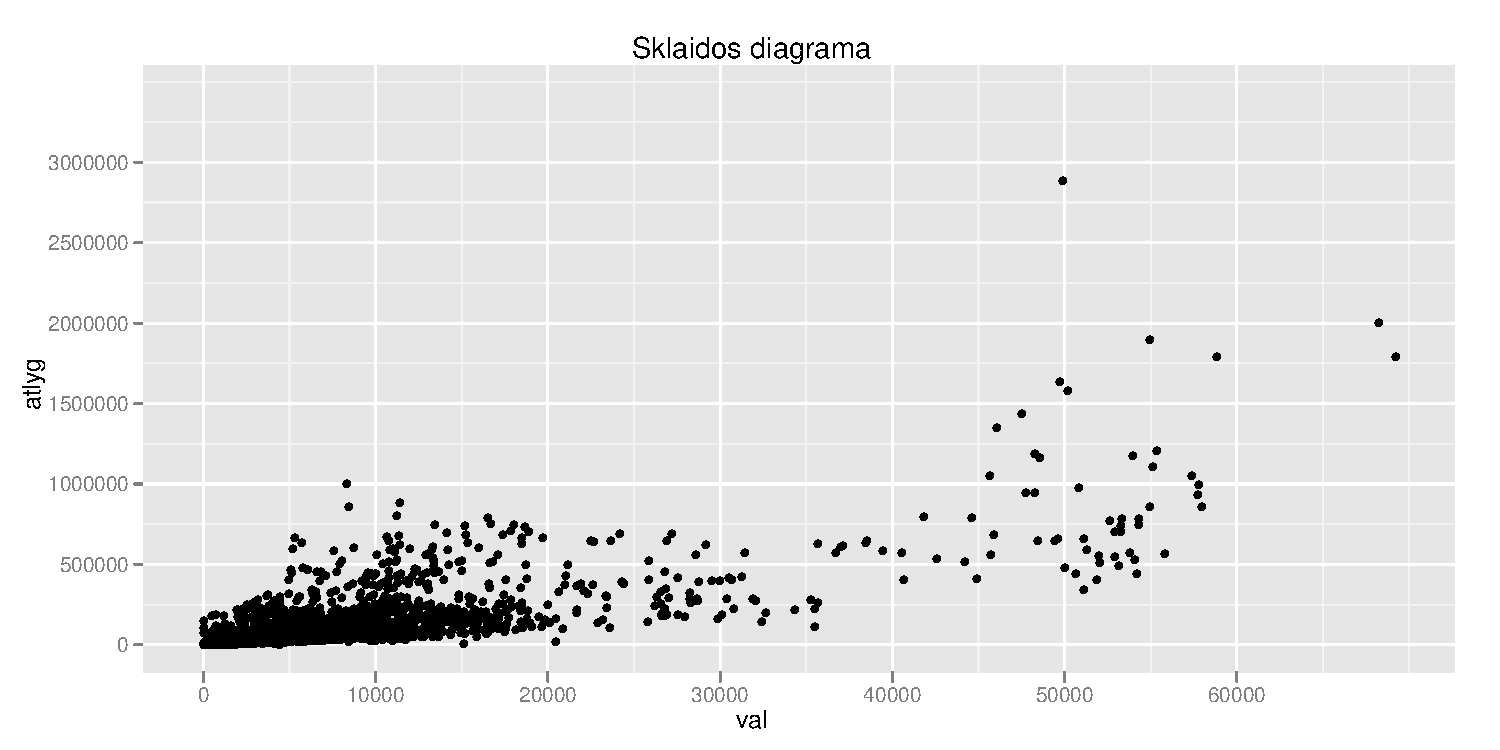
\includegraphics[height=8.5cm]{val_atlyg.pdf}
\caption{Kintamųjų $val$ ir $atlyg$ sklaidos diagrama}
\label{fig:valatlyg}
\end{figure}

\begin{figure}[here]
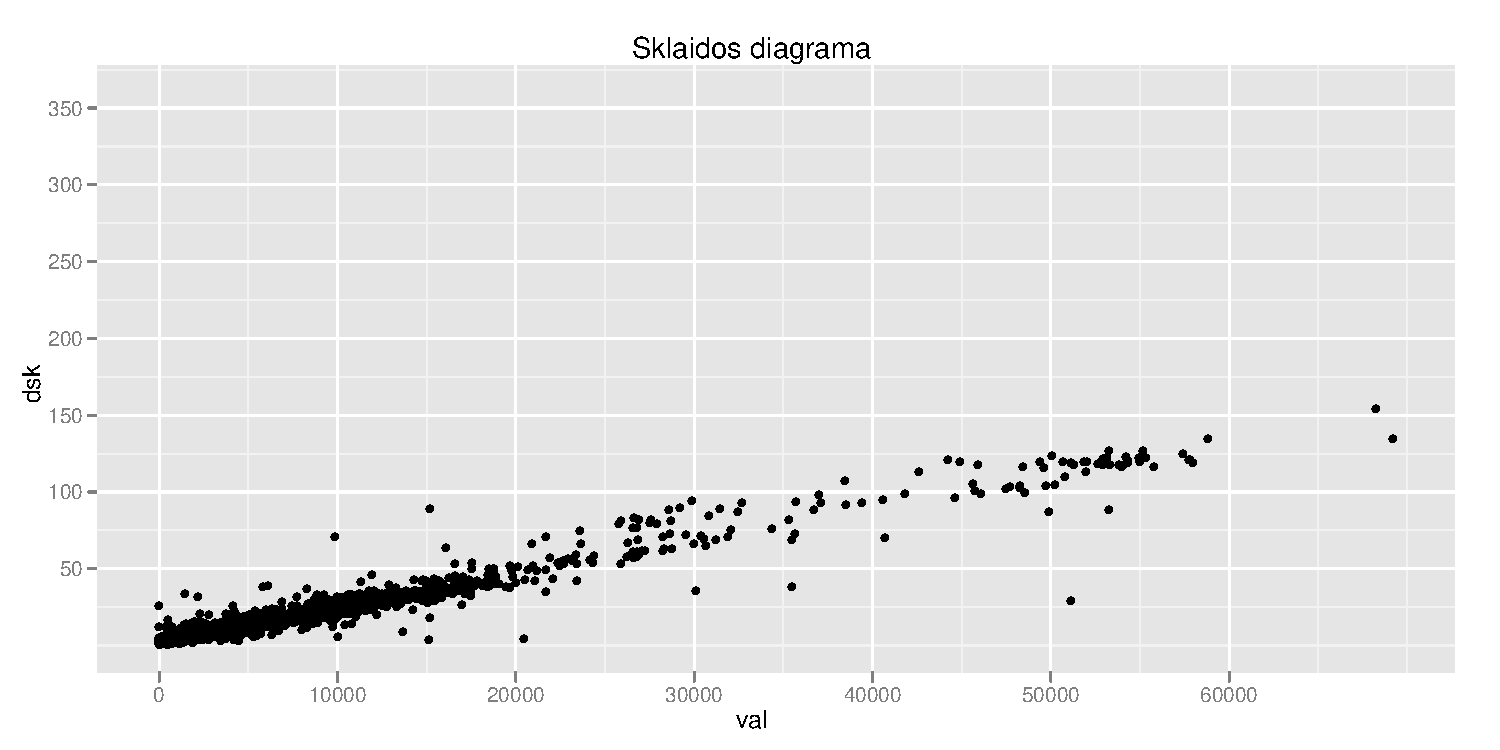
\includegraphics[height=8.5cm]{val_dsk.pdf}
\caption{Kintamųjų $val$ ir $dsk$ sklaidos diagrama}
\label{fig:valdsk}
\end{figure}

Iš viso turima 1430 įmonių priklausančių trečiai grupei, tačiau domina
tik tos, kurių rodiklis $val$ turi bent viena reikšmę per visus metus.
Kitu atveju, duomenys nesuteiks naudingos informacijos. Tokių įmonių
yra 651:
\begin{Schunk}
\begin{Soutput}
  [1]   530   544   552   570   571   574   577   580   591   607   629   683
 [13]   729   743   748   750   757   807   815   875   889   949  1088  1099
 [25]  1128  1193  1195  1208  1209  1241  1264  1272  1291  1306  1307  1337
 [37]  1346  1405  1433  1489  1514  1560  1590  1596  1602  1655  1661  1668
 [49]  1672  1687  1708  1765  1794  1825  1845  1872  1887  1896  1901  1918
 [61]  1941  1944  1945  1947  1966  1967  2095  2113  2116  2137  2145  2153
 [73]  2156  2157  2174  2177  2189  2200  2215  2249  2254  2256  2259  2266
 [85]  2267  2269  2277  2280  2283  2284  2294  2327  2342  2394  2440  2468
 [97]  2491  2508  2530  2596  2697  2707  2708  2725  2727  2799  2813  2867
[109]  2869  2911  2936  2952  2955  2964  2972  2973  2976  2982  2989  3049
[121]  3139  3165  3181  3200  3203  3206  3208  3230  3305  3313  3351  3361
[133]  3362  3366  3368  3374  3375  3398  3401  3440  3469  3528  3585  3607
[145]  3632  3649  3657  3660  3670  3681  3682  3683  3685  3687  3690  3693
[157]  3696  3731  3759  3761  3789  3795  3830  3896  3942  3972  3978  3988
[169]  3995  4004  4006  4009  4036  4040  4055  4062  4063  4064  4065  4078
[181]  4085  4090  4091  4099  4100  4101  4108  4112  4119  4122  4152  4190
[193]  4229  4243  4273  4325  4455  4481  4483  4517  4533  4564  4574  4591
[205]  4603  4636  4639  4646  4647  4648  4650  4651  4652  4654  4681  4686
[217]  4687  4708  4722  4734  4735  4737  4741  4747  4760  4761  4763  4765
[229]  4775  4776  4779  4791  4800  4807  4818  4820  4824  4847  4853  4867
[241]  4870  4873  4886  4889  4892  4894  4896  4899  4901  4904  4906  4908
[253]  4917  4918  4919  4924  4925  4947  4963  4968  4973  4979  5029  5052
[265]  5053  5057  5060  5116  5118  5151  5162  5169  5175  5212  5224  5228
[277]  5280  5290  5338  5400  5411  5428  5442  5457  5477  5501  5553  5573
[289]  5587  5609  5644  5645  5660  5709  5716  5736  5757  5760  5766  5778
[301]  5802  5825  5840  5845  5896  5903  5904  5971  5992  6012  6024  6025
[313]  6044  6050  6053  6061  6062  6074  6077  6080  6093  6094  6099  6101
[325]  6103  6139  6148  6151  6152  6160  6163  6167  6168  6170  6175  6178
[337]  6179  6182  6190  6200  6201  6206  6209  6214  6218  6245  6248  6251
[349]  6255  6270  6282  6285  6316  6318  6325  6326  6334  6337  6338  6348
[361]  6355  6361  6385  6390  6411  6424  6438  6445  6459  6462  6464  6486
[373]  6534  6539  6542  6548  6554  6570  6571  6592  6641  6653  6746  6768
[385]  6784  6847  6907  6914  7056  7074  7090  7123  7139  7199  7245  7265
[397]  7357  7385  7425  7455  7509  7510  7529  7688  7761  7767  7838  7845
[409]  7868  7887  7889  7890  7954  7955  8017  8020  8041  8068  8073  8085
[421]  8105  8120  8136  8143  8145  8148  8152  8162  8183  8224  8240  8246
[433]  8266  8302  8361  8409  8411  8442  8475  8477  8483  8485  8544  8554
[445]  8588  8594  8605  8643  8694  8700  8733  8734  8740  8742  8766  8769
[457]  8787  8794  8853  8860  8864  8869  8896  8917  8937  8947  8962  8968
[469]  8974  8975  8979  9001  9002  9006  9007  9029  9034  9049  9074  9079
[481]  9087  9088  9089  9090  9096  9103  9112  9114  9120  9122  9129  9145
[493]  9147  9152  9153  9158  9164  9178  9182  9184  9185  9186  9191  9193
[505]  9195  9202  9213  9214  9216  9245  9250  9257  9262  9263  9266  9267
[517]  9277  9278  9281  9282  9284  9310  9336  9341  9356  9391  9400  9413
[529]  9414  9417  9421  9427  9428  9431  9435  9450  9480  9491  9492  9495
[541]  9501  9516  9519  9541  9542  9543  9547  9554  9578  9598  9610  9628
[553]  9630  9631  9674  9683  9684  9716  9718  9731  9733  9753  9754  9760
[565]  9774  9775  9782  9787  9799  9804  9856  9868  9870  9893  9908 10008
[577] 10017 10051 10057 10092 10122 10149 10166 10167 10204 10206 10263 10265
[589] 10285 10311 10320 10350 10381 10398 10416 10440 10465 10477 10492 10535
[601] 10565 10567 10597 10629 10650 10668 10687 10694 10732 10765 10787 10838
[613] 10842 10855 10904 10939 10973 10992 10997 11016 11025 11065 11089 11160
[625] 11167 11283 11374 11382 11409 11438 11452 11468 11489 11612 11707 11720
[637] 11730 11760 11795 11797 11812 11819 11824 11829 11839 11853 11855 11859
[649] 11880 11931 11939
\end{Soutput}
\end{Schunk}
Dabar pagrindinės duomenų charakteristikos atrodo taip:
\begin{Schunk}
\begin{Soutput}
       nr             time          veikla       grupe        paj          
 Min.   :  539   Min.   :2005   Min.   :70   Min.   :3   Min.   :       0  
 1st Qu.: 4819   1st Qu.:2006   1st Qu.:70   1st Qu.:3   1st Qu.:   45000  
 Median : 7187   Median :2007   Median :70   Median :3   Median :  198609  
 Mean   : 6980   Mean   :2007   Mean   :70   Mean   :3   Mean   : 1110513  
 3rd Qu.: 9432   3rd Qu.:2008   3rd Qu.:70   3rd Qu.:3   3rd Qu.:  621630  
 Max.   :11944   Max.   :2009   Max.   :70   Max.   :3   Max.   :68509767  
                                                         NA's   :    5695  
      dsk                val              atlyg              ter        
 Min.   :   0.500   Min.   :    0.0   Min.   :      0   Min.   : 11.00  
 1st Qu.:   2.000   1st Qu.:  711.8   1st Qu.:   4500   1st Qu.: 13.00  
 Median :   4.500   Median : 1808.0   Median :  13916   Median : 18.00  
 Mean   :   8.167   Mean   : 3849.4   Mean   :  43096   Mean   : 21.69  
 3rd Qu.:   9.000   3rd Qu.: 4369.5   3rd Qu.:  40688   3rd Qu.: 21.00  
 Max.   : 154.500   Max.   :69208.0   Max.   :2883086   Max.   : 91.00  
 NA's   :1705.000   NA's   : 5952.0   NA's   :   1705   NA's   :212.00  
     nace1            nace2              t       
 Min.   :452100   Min.   : 24000   Min.   :2005  
 1st Qu.:702000   1st Qu.:682000   1st Qu.:2006  
 Median :702000   Median :682000   Median :2007  
 Mean   :703986   Mean   :657128   Mean   :2007  
 3rd Qu.:702000   3rd Qu.:682000   3rd Qu.:2008  
 Max.   :930500   Max.   :960900   Max.   :2009  
 NA's   :   188   NA's   :   188                 
\end{Soutput}
\end{Schunk}
Kad susidaryčiau aiškesnį vaizdą, kokie yra turimi duomenys,
išsibrėžiau kiekvienos įmonės kiekvieno rodiklio grafikus. Jie
patalpinti šio dokumento prisegtuke \emph{pdf} formatu, pavadinimu
\emph{all\_ind.pdf}. Panašu, jog duomenys turi daug tuščių reikšmių ir
trūkių. Iš pradžių pabandysiu tai ignoruoti ir sudaryti panelinių
duomenų modelį. Taip pat paruošiu kelis duomenų masyvus, t.y. skelsiu
duomenis pagal tuščių reikšmių kiekį bei skaidysiu į grupes. Ir
bandysiu pagerinti rezultatus.

\section{Modeliavimas}
Kaip jau minėta, pradžioje sudarysiu paprastą panelių duomenų
modelį. Kadangi kintamieji $nace1$ ir $nace2$ žymi tą patį tik pagal
skirtingus reikalavimus, pasiliksiu vieną iš jų. Tegul tai būna
$nace2$. Sudarysiu \emph{pooled} panelinių duomenų modelį
(\R{} paketas \emph{plm})duomenims iki 2008 metų:
\begin{Schunk}
\begin{Soutput}
val ~ t + dsk + atlyg + ter + nace1
\end{Soutput}
\end{Schunk}
\begin{Schunk}
\begin{Soutput}
Oneway (individual) effect Pooling Model

Call:
plm(formula = fm, data = model.data, effect = "individual", model = "pooling")

Unbalanced Panel: n=691, T=1-12, N=4702

Residuals :
   Min. 1st Qu.  Median 3rd Qu.    Max. 
 -23000    -342      51     396   38600 

Coefficients :
               Estimate  Std. Error  t-value  Pr(>|t|)    
(Intercept)  1.9181e+05  4.7360e+04   4.0500 5.204e-05 ***
t           -9.5991e+01  2.3602e+01  -4.0670 4.840e-05 ***
dsk          3.9346e+02  2.1132e+00 186.1888 < 2.2e-16 ***
atlyg        4.9017e-03  2.5771e-04  19.0203 < 2.2e-16 ***
ter         -1.1681e+00  1.2337e+00  -0.9469    0.3438    
nace1        5.5020e-04  6.7892e-04   0.8104    0.4177    
---
Signif. codes:  0 '***' 0.001 '**' 0.01 '*' 0.05 '.' 0.1 ' ' 1 

Total Sum of Squares:    2.1153e+11
Residual Sum of Squares: 8591400000
R-Squared      :  0.95938 
      Adj. R-Squared :  0.95816 
F-statistic: 22184.7 on 5 and 4696 DF, p-value: < 2.22e-16
\end{Soutput}
\end{Schunk}
Du kintamieji yra nereikšmingi ($ter$ ir $nace1$), tačiau
jei jie nereikšmingi, jų dydžiai ir neturės reikšmingos įtakos
endogeniniam kintamąjam. Tokių kintamųjų pašalinti nėra prasmės, tuo
labiau, kai nežinoma, ar gautas modelis geras. Gerų rezultatų nerodo
ir paklaidų kvadratų sumos. Dar galima pastebėti, jog laiko įtaka yra
neigiama. Būtų galima logaritmuoti $atlyg$, tačiau šis kintamasis
turi nulinių reikšmių. Pabandžiau įtraukti teritorijos žymimuosius
kintamuosius, tačiau rezultatai tik pablogejo. Taip pat galima bandyti įtraukti sezoninius
žymimuosius kintamuosius. Tai ir padarysiu. Įrauksiu tris žymimuosius
kintamuosius $s2$, $s3$ ir $s4$, kurie žymės antrą, trečią ir ketvirtą
sezonus atitinkamai.
\begin{Schunk}
\begin{Soutput}
val ~ t + s2 + s3 + s4 + dsk + atlyg + ter + nace1
\end{Soutput}
\end{Schunk}
\begin{Schunk}
\begin{Soutput}
Oneway (individual) effect Pooling Model

Call:
plm(formula = fm.s, data = model.data1, effect = "individual", 
    model = "pooling")

Unbalanced Panel: n=691, T=1-12, N=4702

Residuals :
    Min.  1st Qu.   Median  3rd Qu.     Max. 
-22900.0   -337.0     59.6    397.0  38500.0 

Coefficients :
               Estimate  Std. Error  t-value  Pr(>|t|)    
(Intercept)  2.0652e+05  5.0142e+04   4.1187 3.876e-05 ***
t           -1.0330e+02  2.4999e+01  -4.1322 3.656e-05 ***
s2          -9.0789e+01  5.6563e+01  -1.6051  0.108540    
s3          -1.5269e+02  5.7615e+01  -2.6501  0.008073 ** 
s4           7.8624e+01  5.9353e+01   1.3247  0.185337    
dsk          3.9365e+02  2.1100e+00 186.5621 < 2.2e-16 ***
atlyg        4.8759e-03  2.5732e-04  18.9486 < 2.2e-16 ***
ter         -1.2040e+00  1.2315e+00  -0.9776  0.328312    
nace1        5.4479e-04  6.7962e-04   0.8016  0.422815    
---
Signif. codes:  0 '***' 0.001 '**' 0.01 '*' 0.05 '.' 0.1 ' ' 1 

Total Sum of Squares:    2.1153e+11
Residual Sum of Squares: 8554800000
R-Squared      :  0.95956 
      Adj. R-Squared :  0.95772 
F-statistic: 13918.3 on 8 and 4693 DF, p-value: < 2.22e-16
\end{Soutput}
\end{Schunk}
Matome, kad ir $s3$ yra reikšmingas. Nepašalinu ir likusių
kintamųjų. Pabandysiu padaryti šio modelio prognozę. Prognozių
grafikai patalpinti šio dokumento prisegtuke pavadinimu
\emph{Valandos\_prognoze\_skirtumas\_zym.pdf}. Iš paveiklslėlių
matyti, jog gan dažnai prognozė daug nenuklysta nuo realių duomenų
(turint omenyje, jog dirbama su gan dideliais dydžiais). Tačiau yra ir
nemažai atvejų, kai prognozė labai nutolsta nuo realybės. Skirtumai
tarp valandų ir jų prognozės pavaizduoti paveikslėliuose
\ref{fig:skzym} ir \ref{fig:skzymb}. Reikia pastebėti, jog
nepavaizduotos tos reikšmės, kurioms nebuvo realių duomenų, nes
palyginimui jos nereikšmingos. Tačiau taip pat svarbu paminėti, jog
išprognozuotų reikšmių buvo daugiau nei realiųjų.

\begin{figure}[here]
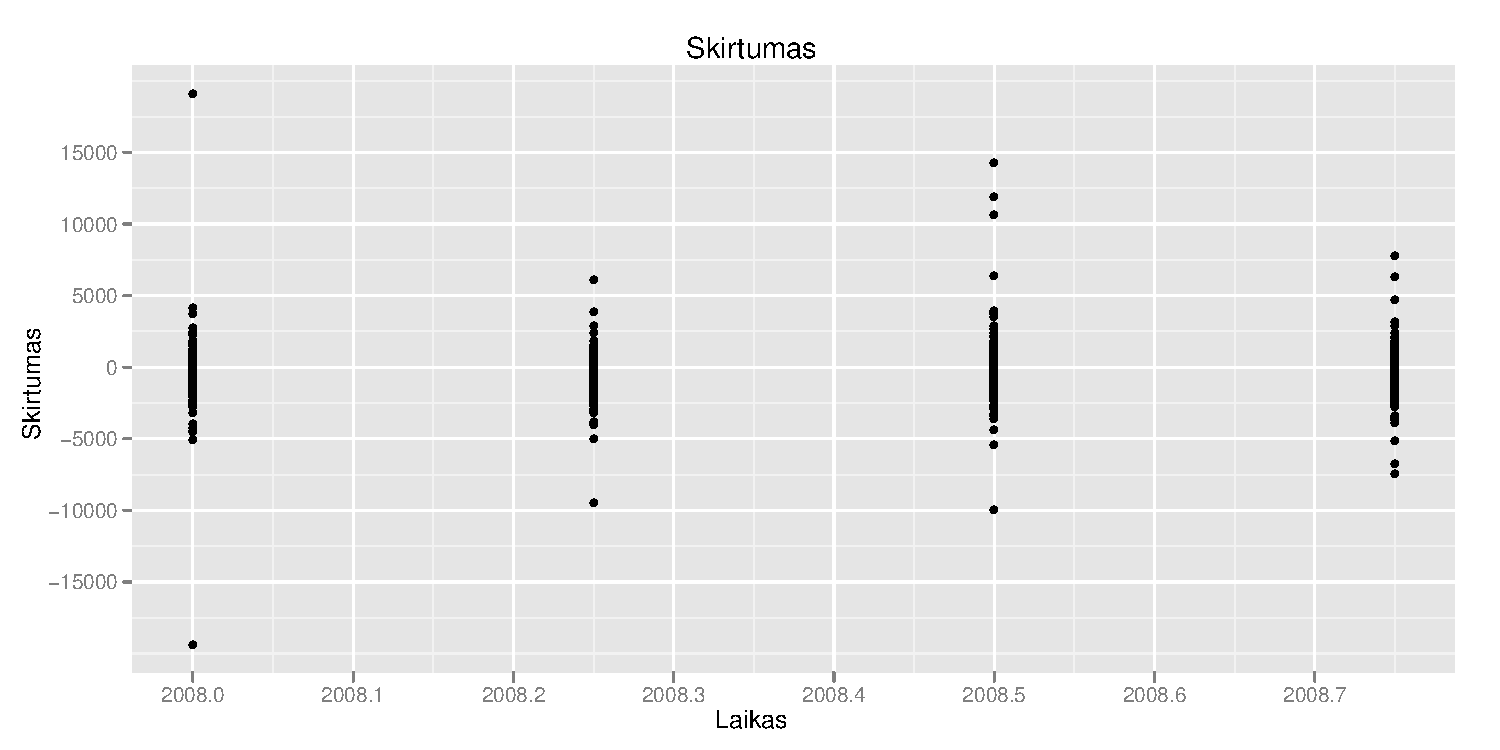
\includegraphics[height=8.5cm]{Skirtumas_zym.pdf}
\caption{Taškais pavaizduotos visų įmonių skirtumai tarp valandų ir
  jų prognozės laike}
\label{fig:skzym}
\end{figure}

\begin{figure}[here]
\includegraphics[height=8.5cm]{Skirtumas_zym_boxplot.pdf}
\caption{Skirtumų tarp valandų ir jų prognozių boxplot}
\label{fig:skzymb}
\end{figure}

Bendras įspūdis nėra blogas, bet pabandysiu prognozes
pagerinti. Kadangi duomenis sudaro įvairaus ilgio valandų laiko eilutės, būtų
galima tokias eilutes skirstyti į ilgesnes ir trumpesnes pagal
kintamąjį $val$. Ilgesnėmis laikysiu eilutes, kurias sudaro bent 4
netuščios reikšmės, visa kita bus laikoma kaip trumpos laiko eilutės. 
Taip pat pastebėjau, jog valandas sudaro ir pastovios
laiko eilutės (konstantos). Konstantas prognozuoti lengva, tam
nereikia sudaryti regresijos, užtenka pratęsti tą pačia reikšmę. Tokių
yra 9:
\begin{Schunk}
\begin{Soutput}
[1]  1368  1574  1735  7050  7537  9331  9836 10632 11429
\end{Soutput}
\end{Schunk}
Jau anksčiau sudarytas modelis, tik ilgesnėms duomenų laiko eilutems:
\begin{Schunk}
\begin{Soutput}
Oneway (individual) effect Pooling Model

Call:
plm(formula = fm.s, data = long, effect = "individual", model = "pooling")

Unbalanced Panel: n=723, T=2-16, N=6153

Residuals :
    Min.  1st Qu.   Median  3rd Qu.     Max. 
-22700.0   -332.0     69.3    412.0  38600.0 

Coefficients :
               Estimate  Std. Error  t-value  Pr(>|t|)    
(Intercept)  1.8737e+05  3.1700e+04   5.9108 3.587e-09 ***
t           -9.3754e+01  1.5797e+01  -5.9351 3.098e-09 ***
s2          -7.6873e+01  4.9169e+01  -1.5634   0.11800    
s3          -1.0511e+02  4.9633e+01  -2.1177   0.03424 *  
s4           8.7291e+01  5.0463e+01   1.7298   0.08372 .  
dsk          3.9628e+02  1.8675e+00 212.1952 < 2.2e-16 ***
atlyg        4.2060e-03  2.1167e-04  19.8709 < 2.2e-16 ***
ter         -9.8901e-01  1.0997e+00  -0.8993   0.36851    
nace1        5.2527e-04  6.3577e-04   0.8262   0.40873    
---
Signif. codes:  0 '***' 0.001 '**' 0.01 '*' 0.05 '.' 0.1 ' ' 1 

Total Sum of Squares:    2.5884e+11
Residual Sum of Squares: 1.125e+10
R-Squared      :  0.95654 
      Adj. R-Squared :  0.95514 
F-statistic: 16903.1 on 8 and 6144 DF, p-value: < 2.22e-16
\end{Soutput}
\end{Schunk}
Rezultatai tik pablogėjo. Nors įmonių skaičius mažesnis, t.y. paklaidų
kvadratų sumos padidėjo.
Nors ir su ilgesnėmis laiko eilutėmis, duomenys vistiek turi labai
daug tuščių reikšmių. Todėl pagalvojau, kad juos galima užpildyti
pasitelkus \R{} f-ją \emph{na.spline}. Rezultatai pateikti
žemiau. Kintamųjų reikšmingumas sumažėjęs ir rezultatai tik pablogėjo.
\begin{Schunk}
\begin{Soutput}
Oneway (individual) effect Pooling Model

Call:
plm(formula = fm.s, data = long.na, effect = "individual", model = "pooling")

Balanced Panel: n=723, T=12, N=8676

Residuals :
   Min. 1st Qu.  Median 3rd Qu.    Max. 
 -23000    -701    -239     268   94400 

Coefficients :
               Estimate  Std. Error t-value Pr(>|t|)    
(Intercept) -2.1065e+04  8.7935e+04 -0.2395   0.8107    
t            1.0869e+01  4.3833e+01  0.2480   0.8042    
s2          -2.2560e+01  1.0172e+02 -0.2218   0.8245    
s3          -3.5925e+01  1.0366e+02 -0.3466   0.7289    
s4           1.0037e+02  1.0649e+02  0.9426   0.3459    
dsk          3.7582e+02  4.2400e+00 88.6369   <2e-16 ***
atlyg        6.4654e-03  4.6738e-04 13.8333   <2e-16 ***
ter         -3.2631e+00  2.2504e+00 -1.4500   0.1471    
nace1       -1.0060e-03  1.3448e-03 -0.7481   0.4544    
---
Signif. codes:  0 '***' 0.001 '**' 0.01 '*' 0.05 '.' 0.1 ' ' 1 

Total Sum of Squares:    3.2084e+11
Residual Sum of Squares: 9.6131e+10
R-Squared      :  0.70037 
      Adj. R-Squared :  0.69965 
F-statistic: 2532.35 on 8 and 8667 DF, p-value: < 2.22e-16
\end{Soutput}
\end{Schunk}
Taip pat tą patį modelį pritaikiau ir trumpoms laiko eilutėms:
\begin{Schunk}
\begin{Soutput}
Oneway (individual) effect Pooling Model

Call:
plm(formula = fm.s, data = short, effect = "individual", model = "pooling")

Unbalanced Panel: n=45, T=1-7, N=216

Residuals :
   Min. 1st Qu.  Median 3rd Qu.    Max. 
-4090.0  -487.0   -40.8   317.0 13400.0 

Coefficients :
               Estimate  Std. Error t-value Pr(>|t|)    
(Intercept)  5.4537e+04  2.3085e+05  0.2362  0.81348    
t           -2.6654e+01  1.1493e+02 -0.2319  0.81684    
s2           4.1659e+01  3.5548e+02  0.1172  0.90682    
s3           1.7546e+02  3.5575e+02  0.4932  0.62239    
s4          -3.8530e+01  3.6090e+02 -0.1068  0.91508    
dsk          3.8532e+02  2.3039e+01 16.7249  < 2e-16 ***
atlyg        3.8330e-03  2.9308e-03  1.3079  0.19237    
ter          1.4844e+01  7.2532e+00  2.0465  0.04197 *  
nace1       -2.5119e-03  2.9458e-03 -0.8527  0.39481    
---
Signif. codes:  0 '***' 0.001 '**' 0.01 '*' 0.05 '.' 0.1 ' ' 1 

Total Sum of Squares:    2809100000
Residual Sum of Squares: 414530000
R-Squared      :  0.85244 
      Adj. R-Squared :  0.81692 
F-statistic: 149.472 on 8 and 207 DF, p-value: < 2.22e-16
\end{Soutput}
\end{Schunk}
Rezultatai taip pat nieko gero nežada. Bet ir nėra, ko norėti, kai
laiko eilutės trumpesnės negu 4.
Dar pabandysiu pagerinti ilgesniųjų laiko eilučių prognozes. Skaidysiu
duomenis į keles grupes pagal įmonių dydį, t.y. $dsk$. Tai darysiu
pagal histogramą \ref. Pirmąją grupę sudarys įmonės su mažesniu nei 5
darbuotojų skaičiumi, antrąją -- 5:10  darbuotojų, trečiąją -- 10:20,
ketvirtąją -- 20:40 ir penktąją įmonės su 40 ir daugiau darbuotojų.

\begin{figure}[here]
\includegraphics[height=8.5cm]{hist_dsk.pdf}
\caption{Ilgesniųjų laiko eilučių darbuotojų skaičiaus histograma}
\label{fig:histdsk}
\end{figure}
\begin{Schunk}
\begin{Soutput}
$gr1
$gr1$Summary
Oneway (individual) effect Pooling Model

Call:
plm(formula = fm.s, data = datt, effect = "individual", model = "pooling")

Unbalanced Panel: n=376, T=2-16, N=2626

Residuals :
   Min. 1st Qu.  Median 3rd Qu.    Max. 
-1740.0  -211.0   -20.5   208.0  3670.0 

Coefficients :
               Estimate  Std. Error t-value  Pr(>|t|)    
(Intercept)  9.3500e+04  1.3626e+04  6.8619 8.450e-12 ***
t           -4.6940e+01  6.7891e+00 -6.9141 5.894e-12 ***
s2           5.5413e+00  2.1305e+01  0.2601   0.79481    
s3           1.6915e+01  2.1506e+01  0.7865   0.43164    
s4           2.2854e+01  2.1874e+01  1.0448   0.29620    
dsk          3.3360e+02  5.7455e+00 58.0625 < 2.2e-16 ***
atlyg        7.3894e-03  5.1654e-04 14.3056 < 2.2e-16 ***
ter          4.7941e-01  4.5031e-01  1.0646   0.28715    
nace1        6.7825e-04  3.2355e-04  2.0963   0.03615 *  
---
Signif. codes:  0 '***' 0.001 '**' 0.01 '*' 0.05 '.' 0.1 ' ' 1 

Total Sum of Squares:    1160700000
Residual Sum of Squares: 382100000
R-Squared      :  0.6708 
      Adj. R-Squared :  0.6685 
F-statistic: 666.575 on 8 and 2617 DF, p-value: < 2.22e-16

$gr1$plm

Model Formula: val ~ t + s2 + s3 + s4 + dsk + atlyg + ter + nace1
<environment: 0x0595e908>

Coefficients:
(Intercept)           t          s2          s3          s4         dsk 
 9.3500e+04 -4.6940e+01  5.5413e+00  1.6915e+01  2.2854e+01  3.3360e+02 
      atlyg         ter       nace1 
 7.3894e-03  4.7941e-01  6.7825e-04 



$gr2
$gr2$Summary
Oneway (individual) effect Pooling Model

Call:
plm(formula = fm.s, data = datt, effect = "individual", model = "pooling")

Unbalanced Panel: n=184, T=3-16, N=1591

Residuals :
   Min. 1st Qu.  Median 3rd Qu.    Max. 
-3650.0  -456.0    22.2   414.0 19000.0 

Coefficients :
               Estimate  Std. Error t-value  Pr(>|t|)    
(Intercept)  1.1930e+05  4.1044e+04  2.9067  0.003703 ** 
t           -5.8900e+01  2.0447e+01 -2.8807  0.004022 ** 
s2          -7.3866e+01  6.2538e+01 -1.1811  0.237724    
s3          -1.0345e+02  6.3342e+01 -1.6332  0.102626    
s4          -4.7733e+01  6.4393e+01 -0.7413  0.458640    
dsk          3.4963e+02  8.7209e+00 40.0907 < 2.2e-16 ***
atlyg        4.2306e-03  5.4317e-04  7.7887 1.216e-14 ***
ter         -1.3116e-01  1.5076e+00 -0.0870  0.930684    
nace1       -1.7381e-03  6.9145e-04 -2.5137  0.012046 *  
---
Signif. codes:  0 '***' 0.001 '**' 0.01 '*' 0.05 '.' 0.1 ' ' 1 

Total Sum of Squares:    2.979e+09
Residual Sum of Squares: 1.209e+09
R-Squared      :  0.59414 
      Adj. R-Squared :  0.59078 
F-statistic: 289.489 on 8 and 1582 DF, p-value: < 2.22e-16

$gr2$plm

Model Formula: val ~ t + s2 + s3 + s4 + dsk + atlyg + ter + nace1
<environment: 0x0940d5c8>

Coefficients:
(Intercept)           t          s2          s3          s4         dsk 
 1.1930e+05 -5.8900e+01 -7.3866e+01 -1.0345e+02 -4.7733e+01  3.4963e+02 
      atlyg         ter       nace1 
 4.2306e-03 -1.3116e-01 -1.7381e-03 



$gr3
$gr3$Summary
Oneway (individual) effect Pooling Model

Call:
plm(formula = fm.s, data = datt, effect = "individual", model = "pooling")

Unbalanced Panel: n=109, T=4-16, N=1144

Residuals :
   Min. 1st Qu.  Median 3rd Qu.    Max. 
 -11000    -585     115     661   10800 

Coefficients :
               Estimate  Std. Error t-value  Pr(>|t|)    
(Intercept)  3.9987e+05  7.1323e+04  5.6065 2.591e-08 ***
t           -2.0069e+02  3.5538e+01 -5.6473 2.059e-08 ***
s2          -2.3887e+01  1.0599e+02 -0.2254 0.8217325    
s3          -9.3326e+01  1.0690e+02 -0.8730 0.3828228    
s4           1.1523e+02  1.0876e+02  1.0595 0.2896002    
dsk          3.6515e+02  8.3592e+00 43.6826 < 2.2e-16 ***
atlyg        3.6259e-03  5.3138e-04  6.8236 1.442e-11 ***
ter         -7.8089e+00  2.1531e+00 -3.6269 0.0002996 ***
nace1        4.0885e-03  1.3426e-03  3.0453 0.0023779 ** 
---
Signif. codes:  0 '***' 0.001 '**' 0.01 '*' 0.05 '.' 0.1 ' ' 1 

Total Sum of Squares:    6.241e+09
Residual Sum of Squares: 1811500000
R-Squared      :  0.70975 
      Adj. R-Squared :  0.70416 
F-statistic: 346.924 on 8 and 1135 DF, p-value: < 2.22e-16

$gr3$plm

Model Formula: val ~ t + s2 + s3 + s4 + dsk + atlyg + ter + nace1
<environment: 0x0504e36c>

Coefficients:
(Intercept)           t          s2          s3          s4         dsk 
 3.9987e+05 -2.0069e+02 -2.3887e+01 -9.3326e+01  1.1523e+02  3.6515e+02 
      atlyg         ter       nace1 
 3.6259e-03 -7.8089e+00  4.0885e-03 



$gr4
$gr4$Summary
Oneway (individual) effect Pooling Model

Call:
plm(formula = fm.s, data = datt, effect = "individual", model = "pooling")

Unbalanced Panel: n=44, T=9-16, N=640

Residuals :
    Min.  1st Qu.   Median  3rd Qu.     Max. 
-11000.0   -918.0     83.4    948.0  38400.0 

Coefficients :
               Estimate  Std. Error t-value Pr(>|t|)    
(Intercept)  1.7173e+05  1.8129e+05  0.9473  0.34387    
t           -8.7030e+01  9.0339e+01 -0.9634  0.33573    
s2          -2.4933e+02  2.6864e+02 -0.9281  0.35370    
s3          -5.0674e+02  2.7132e+02 -1.8677  0.06227 .  
s4           5.4017e+02  2.7506e+02  1.9638  0.04999 *  
dsk          4.2566e+02  1.0577e+01 40.2453  < 2e-16 ***
atlyg        1.5370e-03  7.2438e-04  2.1218  0.03424 *  
ter          1.4305e+01  8.6257e+00  1.6584  0.09773 .  
nace1        2.9507e-03  3.2173e-03  0.9171  0.35942    
---
Signif. codes:  0 '***' 0.001 '**' 0.01 '*' 0.05 '.' 0.1 ' ' 1 

Total Sum of Squares:    1.5105e+10
Residual Sum of Squares: 3580600000
R-Squared      :  0.76295 
      Adj. R-Squared :  0.75223 
F-statistic: 253.866 on 8 and 631 DF, p-value: < 2.22e-16

$gr4$plm

Model Formula: val ~ t + s2 + s3 + s4 + dsk + atlyg + ter + nace1
<environment: 0x029f4148>

Coefficients:
(Intercept)           t          s2          s3          s4         dsk 
 1.7173e+05 -8.7030e+01 -2.4933e+02 -5.0674e+02  5.4017e+02  4.2566e+02 
      atlyg         ter       nace1 
 1.5370e-03  1.4305e+01  2.9507e-03 



$gr5
$gr5$Summary
Oneway (individual) effect Pooling Model

Call:
plm(formula = fm.s, data = datt, effect = "individual", model = "pooling")

Unbalanced Panel: n=10, T=12-16, N=152

Residuals :
   Min. 1st Qu.  Median 3rd Qu.    Max. 
 -22900   -1850     346    1890   20500 

Coefficients :
               Estimate  Std. Error t-value  Pr(>|t|)    
(Intercept)  8.9031e+05  9.3180e+05  0.9555  0.340949    
t           -5.3493e+02  4.0479e+02 -1.3215  0.188444    
s2          -1.4006e+03  1.1034e+03 -1.2693  0.206381    
s3          -8.4022e+02  1.1528e+03 -0.7289  0.467267    
s4           2.7847e+02  1.1649e+03  0.2390  0.811418    
dsk          4.1116e+02  1.5958e+01 25.7653 < 2.2e-16 ***
atlyg        6.0684e-03  1.2279e-03  4.9420 2.134e-06 ***
ter         -2.1521e+02  7.7158e+01 -2.7892  0.006004 ** 
nace1        2.6250e-01  8.3571e-01  0.3141  0.753896    
---
Signif. codes:  0 '***' 0.001 '**' 0.01 '*' 0.05 '.' 0.1 ' ' 1 

Total Sum of Squares:    3.9656e+10
Residual Sum of Squares: 3273400000
R-Squared      :  0.91746 
      Adj. R-Squared :  0.86313 
F-statistic: 198.676 on 8 and 143 DF, p-value: < 2.22e-16

$gr5$plm

Model Formula: val ~ t + s2 + s3 + s4 + dsk + atlyg + ter + nace1
<environment: 0x04fb1050>

Coefficients:
(Intercept)           t          s2          s3          s4         dsk 
 8.9031e+05 -5.3493e+02 -1.4006e+03 -8.4022e+02  2.7847e+02  4.1116e+02 
      atlyg         ter       nace1 
 6.0684e-03 -2.1521e+02  2.6250e-01 
\end{Soutput}
\end{Schunk}
Padariusi prognozes ir suskaičiavusi jų skirtumą nuo realių darbo
valandų, gavau, jog skaidymas į grupes pagerino absoliutinių skirtumų
sumą, t.y:
\begin{Schunk}
\begin{Sinput}
> sum(abs(errors.long$Skirtumas), na.rm = TRUE)
\end{Sinput}
\begin{Soutput}
[1] 1093791
\end{Soutput}
\begin{Sinput}
> sum(abs(errors.gr$Skirtumas), na.rm = TRUE)
\end{Sinput}
\begin{Soutput}
[1] 993769.5
\end{Soutput}
\end{Schunk}
Dar bandžiau padaryti paprastą tiesinę regresiją kiekvienai įmonei
atskirai. Tačiau geresnių rezultatų gauti nepavyko. Galutines
prognozes, bei skirtumus nuo realių valandų galima pamatyti šio
dokumento prisegtuke pavadinimu \emph{Prognozes.csv}.

\section{Išvados}
Labai gerų rezultatų gauti nepavyko. To priežąstys gali būti:
\begin{itemize}
  \item blogai sudarytas modelis
  \item per didelė įmonių įvairovė
  \item pasirinkti ne tie metodai
  \item ir k.t.
\end{itemize}

\end{document}
